\documentclass{article}
\usepackage[utf8]{inputenc}
\usepackage{ragged2e}
\usepackage{graphicx}
\usepackage{float}

\title{Práctica2}
\author{Enrique Narbona Luque}
\date{October 2022}

\begin{document}

\maketitle

\LARGE
\titl\underline{Actividades}

\vspace{4mm}

\normalsize
\RaggedRight

\textbf{1. Consider the language over the alphabet \{a, b\} that only contains the string a.}

\vspace{4mm}

\textbf{a. Build a DFA that recognizes this language and rejects all those strings that do not belong to the language.}

\vspace{5mm}

Un autómata finito determinista (DFA) es una 5-tupla(K,\sum,\delta,s,F) donde:

\vspace{4mm}

K es un conjunto de estados no vacíos

\vspace{4mm}

\sum es un alfabeto

\vspace{4mm}

s \in K es el estado inicial

\vspace{4mm}

F \subseteq K es el conjunto de estados finales

\vspace{4mm}

\delta : K \times \sum \rightarrow K es la función de transición

\vspace{4mm}

\newpage
\RaggedRight

Un ejemplo de DFA que reconozca el lenguaje pedido es:

\vspace{3mm}

\centering{M = (\{q_{0},q_{1}\},\{a,b\},\delta,\{q_{0}\})}

\vspace{5mm}

\begin{figure}[htb]
    \centering
    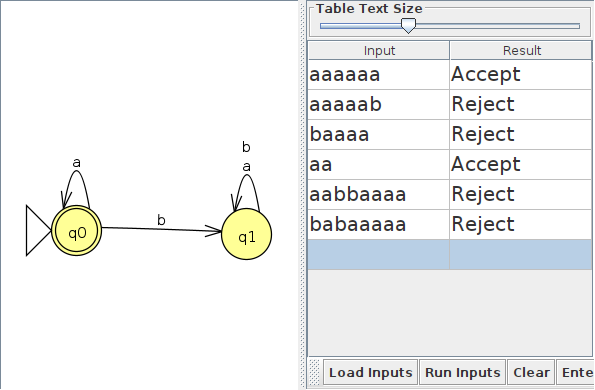
\includegraphics[scale = 0.5]{DFA_Practica 2.png}
    \label{DFA_Practica 2.png}
\end{figure}

\vspace{6mm}

\RaggedRight
\textbf{b. Test the automaton that you have created by introducing 6 chains.}

\vspace{5mm}

\begin{figure}[htb]
    \centering
    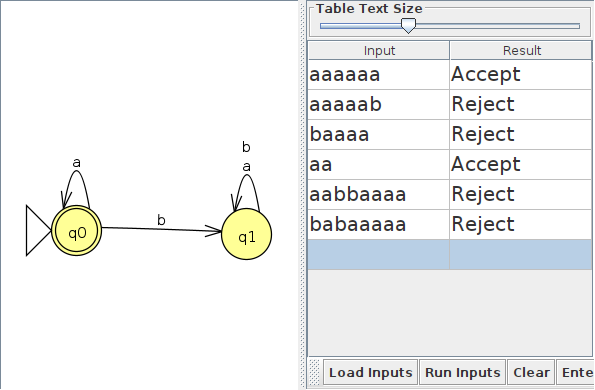
\includegraphics[scale = 0.5]{DFA_Practica 2.png}
    \label{DFA_Practica 2.png}
\end{figure}

\newpage

\normalsize
\RaggedRight

\textbf{2. Finite automaton in Octave:}

\vspace{4mm}

\textbf{a. Open the Octave finiteautomata.m script and test it with the given
example (see script help) in the GitHub repository.}

\vspace{4mm}

\textbf{b. Specify in finiteautomata.json the automaton created in Activity 1
and test it with the script!}

\vspace{4mm}

\begin{verbatim}
    {
    "name" : "a*",
    "representation" : {
      "K" : ["q0", "q1"],
      "A" : ["a", "b"],
      "s" : "q0",
      "F" : ["q0"],
      "t" : [["q0", "a", "q0"],
             ["q0", "b", "q1"],
             ["q1", "a", "q1"],
             ["q1", "b", "q1"]]
      }
    }
\end{verbatim}

\end{document}